
%% bare_conf.tex
%% V1.3
%% 2007/01/11
%% by Michael Shell
%% See:
%% http://www.michaelshell.org/
%% for current contact information.
%%
%% This is a skeleton file demonstrating the use of IEEEtran.cls
%% (requires IEEEtran.cls version 1.7 or later) with an IEEE conference paper.
%%
%% Support sites:
%% http://www.michaelshell.org/tex/ieeetran/
%% http://www.ctan.org/tex-archive/macros/latex/contrib/IEEEtran/
%% and
%% http://www.ieee.org/

%%*************************************************************************
%% Legal Notice:
%% This code is offered as-is without any warranty either expressed or
%% implied; without even the implied warranty of MERCHANTABILITY or
%% FITNESS FOR A PARTICULAR PURPOSE! 
%% User assumes all risk.
%% In no event shall IEEE or any contributor to this code be liable for
%% any damages or losses, including, but not limited to, incidental,
%% consequential, or any other damages, resulting from the use or misuse
%% of any information contained here.
%%
%% All comments are the opinions of their respective authors and are not
%% necessarily endorsed by the IEEE.
%%
%% This work is distributed under the LaTeX Project Public License (LPPL)
%% ( http://www.latex-project.org/ ) version 1.3, and may be freely used,
%% distributed and modified. A copy of the LPPL, version 1.3, is included
%% in the base LaTeX documentation of all distributions of LaTeX released
%% 2003/12/01 or later.
%% Retain all contribution notices and credits.
%% ** Modified files should be clearly indicated as such, including  **
%% ** renaming them and changing author support contact information. **
%%
%% File list of work: IEEEtran.cls, IEEEtran_HOWTO.pdf, bare_adv.tex,
%%                    bare_conf.tex, bare_jrnl.tex, bare_jrnl_compsoc.tex
%%*************************************************************************

% *** Authors should verify (and, if needed, correct) their LaTeX system  ***
% *** with the testflow diagnostic prior to trusting their LaTeX platform ***
% *** with production work. IEEE's font choices can trigger bugs that do  ***
% *** not appear when using other class files.                            ***
% The testflow support page is at:
% http://www.michaelshell.org/tex/testflow/



% Note that the a4paper option is mainly intended so that authors in
% countries using A4 can easily print to A4 and see how their papers will
% look in print - the typesetting of the document will not typically be
% affected with changes in paper size (but the bottom and side margins will).
% Use the testflow package mentioned above to verify correct handling of
% both paper sizes by the user's LaTeX system.
%
% Also note that the "draftcls" or "draftclsnofoot", not "draft", option
% should be used if it is desired that the figures are to be displayed in
% draft mode.
%
\documentclass[10pt, conference, compsocconf]{IEEEtran}
% Add the compsocconf option for Computer Society conferences.
%
% If IEEEtran.cls has not been installed into the LaTeX system files,
% manually specify the path to it like:
% \documentclass[conference]{../sty/IEEEtran}





% Some very useful LaTeX packages include:
% (uncomment the ones you want to load)


% *** MISC UTILITY PACKAGES ***
%
%\usepackage{ifpdf}
% Heiko Oberdiek's ifpdf.sty is very useful if you need conditional
% compilation based on whether the output is pdf or dvi.
% usage:
% \ifpdf
%   % pdf code
% \else
%   % dvi code
% \fi
% The latest version of ifpdf.sty can be obtained from:
% http://www.ctan.org/tex-archive/macros/latex/contrib/oberdiek/
% Also, note that IEEEtran.cls V1.7 and later provides a builtin
% \ifCLASSINFOpdf conditional that works the same way.
% When switching from latex to pdflatex and vice-versa, the compiler may
% have to be run twice to clear warning/error messages.






% *** CITATION PACKAGES ***
%
%\usepackage{cite}
% cite.sty was written by Donald Arseneau
% V1.6 and later of IEEEtran pre-defines the format of the cite.sty package
% \cite{} output to follow that of IEEE. Loading the cite package will
% result in citation numbers being automatically sorted and properly
% "compressed/ranged". e.g., [1], [9], [2], [7], [5], [6] without using
% cite.sty will become [1], [2], [5]--[7], [9] using cite.sty. cite.sty's
% \cite will automatically add leading space, if needed. Use cite.sty's
% noadjust option (cite.sty V3.8 and later) if you want to turn this off.
% cite.sty is already installed on most LaTeX systems. Be sure and use
% version 4.0 (2003-05-27) and later if using hyperref.sty. cite.sty does
% not currently provide for hyperlinked citations.
% The latest version can be obtained at:
% http://www.ctan.org/tex-archive/macros/latex/contrib/cite/
% The documentation is contained in the cite.sty file itself.



\usepackage{arydshln}

%\usepackage{pdfpages}


% *** GRAPHICS RELATED PACKAGES ***
%
\ifCLASSINFOpdf
  \usepackage[pdftex]{graphicx}
  % declare the path(s) where your graphic files are
  \graphicspath{{../pdf/}{../jpeg/}}
  % and their extensions so you won't have to specify these with
  % every instance of \includegraphics
  \DeclareGraphicsExtensions{.pdf,.jpeg,.png}
\else
  % or other class option (dvipsone, dvipdf, if not using dvips). graphicx
  % will default to the driver specified in the system graphics.cfg if no
  % driver is specified.
  \usepackage[dvips]{graphicx}
  % declare the path(s) where your graphic files are
  \graphicspath{{../eps/}}
  % and their extensions so you won't have to specify these with
  % every instance of \includegraphics
  \DeclareGraphicsExtensions{.eps}
\fi
% graphicx was written by David Carlisle and Sebastian Rahtz. It is
% required if you want graphics, photos, etc. graphicx.sty is already
% installed on most LaTeX systems. The latest version and documentation can
% be obtained at: 
% http://www.ctan.org/tex-archive/macros/latex/required/graphics/
% Another good source of documentation is "Using Imported Graphics in
% LaTeX2e" by Keith Reckdahl which can be found as epslatex.ps or
% epslatex.pdf at: http://www.ctan.org/tex-archive/info/
%
% latex, and pdflatex in dvi mode, support graphics in encapsulated
% postscript (.eps) format. pdflatex in pdf mode supports graphics
% in .pdf, .jpeg, .png and .mps (metapost) formats. Users should ensure
% that all non-photo figures use a vector format (.eps, .pdf, .mps) and
% not a bitmapped formats (.jpeg, .png). IEEE frowns on bitmapped formats
% which can result in "jaggedy"/blurry rendering of lines and letters as
% well as large increases in file sizes.
%
% You can find documentation about the pdfTeX application at:
% http://www.tug.org/applications/pdftex





% *** MATH PACKAGES ***
%
\usepackage[cmex10]{amsmath}
% A popular package from the American Mathematical Society that provides
% many useful and powerful commands for dealing with mathematics. If using
% it, be sure to load this package with the cmex10 option to ensure that
% only type 1 fonts will utilized at all point sizes. Without this option,
% it is possible that some math symbols, particularly those within
% footnotes, will be rendered in bitmap form which will result in a
% document that can not be IEEE Xplore compliant!
%
% Also, note that the amsmath package sets \interdisplaylinepenalty to 10000
% thus preventing page breaks from occurring within multiline equations. Use:
%\interdisplaylinepenalty=2500
% after loading amsmath to restore such page breaks as IEEEtran.cls normally
% does. amsmath.sty is already installed on most LaTeX systems. The latest
% version and documentation can be obtained at:
% http://www.ctan.org/tex-archive/macros/latex/required/amslatex/math/
\usepackage{romannum}


\usepackage{algorithm}
\usepackage[algo2e]{algorithm2e}
% *** SPECIALIZED LIST PACKAGES ***
%
%\usepackage{algorithmic}
% algorithmic.sty was written by Peter Williams and Rogerio Brito.
% This package provides an algorithmic environment fo describing algorithms.
% You can use the algorithmic environment in-text or within a figure
% environment to provide for a floating algorithm. Do NOT use the algorithm
% floating environment provided by algorithm.sty (by the same authors) or
% algorithm2e.sty (by Christophe Fiorio) as IEEE does not use dedicated
% algorithm float types and packages that provide these will not provide
% correct IEEE style captions. The latest version and documentation of
% algorithmic.sty can be obtained at:
% http://www.ctan.org/tex-archive/macros/latex/contrib/algorithms/
% There is also a support site at:
% http://algorithms.berlios.de/index.html
% Also of interest may be the (relatively newer and more customizable)
% algorithmicx.sty package by Szasz Janos:
% http://www.ctan.org/tex-archive/macros/latex/contrib/algorithmicx/




% *** ALIGNMENT PACKAGES ***
%
%\usepackage{array}
% Frank Mittelbach's and David Carlisle's array.sty patches and improves
% the standard LaTeX2e array and tabular environments to provide better
% appearance and additional user controls. As the default LaTeX2e table
% generation code is lacking to the point of almost being broken with
% respect to the quality of the end results, all users are strongly
% advised to use an enhanced (at the very least that provided by array.sty)
% set of table tools. array.sty is already installed on most systems. The
% latest version and documentation can be obtained at:
% http://www.ctan.org/tex-archive/macros/latex/required/tools/


%\usepackage{mdwmath}
%\usepackage{mdwtab}
% Also highly recommended is Mark Wooding's extremely powerful MDW tools,
% especially mdwmath.sty and mdwtab.sty which are used to format equations
% and tables, respectively. The MDWtools set is already installed on most
% LaTeX systems. The lastest version and documentation is available at:
% http://www.ctan.org/tex-archive/macros/latex/contrib/mdwtools/


% IEEEtran contains the IEEEeqnarray family of commands that can be used to
% generate multiline equations as well as matrices, tables, etc., of high
% quality.


%\usepackage{eqparbox}
% Also of notable interest is Scott Pakin's eqparbox package for creating
% (automatically sized) equal width boxes - aka "natural width parboxes".
% Available at:
% http://www.ctan.org/tex-archive/macros/latex/contrib/eqparbox/





% *** SUBFIGURE PACKAGES ***
%\usepackage[tight,footnotesize]{subfigure}
% subfigure.sty was written by Steven Douglas Cochran. This package makes it
% easy to put subfigures in your figures. e.g., "Figure 1a and 1b". For IEEE
% work, it is a good idea to load it with the tight package option to reduce
% the amount of white space around the subfigures. subfigure.sty is already
% installed on most LaTeX systems. The latest version and documentation can
% be obtained at:
% http://www.ctan.org/tex-archive/obsolete/macros/latex/contrib/subfigure/
% subfigure.sty has been superceeded by subfig.sty.



%\usepackage[caption=false]{caption}
\usepackage[caption=false,font=footnotesize]{subfig}
% subfig.sty, also written by Steven Douglas Cochran, is the modern
% replacement for subfigure.sty. However, subfig.sty requires and
% automatically loads Axel Sommerfeldt's caption.sty which will override
% IEEEtran.cls handling of captions and this will result in nonIEEE style
% figure/table captions. To prevent this problem, be sure and preload
% caption.sty with its "caption=false" package option. This is will preserve
% IEEEtran.cls handing of captions. Version 1.3 (2005/06/28) and later 
% (recommended due to many improvements over 1.2) of subfig.sty supports
% the caption=false option directly:
%\usepackage[caption=false,font=footnotesize]{subfig}
%
% The latest version and documentation can be obtained at:
% http://www.ctan.org/tex-archive/macros/latex/contrib/subfig/
% The latest version and documentation of caption.sty can be obtained at:
% http://www.ctan.org/tex-archive/macros/latex/contrib/caption/




% *** FLOAT PACKAGES ***
%
%\usepackage{fixltx2e}
% fixltx2e, the successor to the earlier fix2col.sty, was written by
% Frank Mittelbach and David Carlisle. This package corrects a few problems
% in the LaTeX2e kernel, the most notable of which is that in current
% LaTeX2e releases, the ordering of single and double column floats is not
% guaranteed to be preserved. Thus, an unpatched LaTeX2e can allow a
% single column figure to be placed prior to an earlier double column
% figure. The latest version and documentation can be found at:
% http://www.ctan.org/tex-archive/macros/latex/base/



%\usepackage{stfloats}
% stfloats.sty was written by Sigitas Tolusis. This package gives LaTeX2e
% the ability to do double column floats at the bottom of the page as well
% as the top. (e.g., "\begin{figure*}[!b]" is not normally possible in
% LaTeX2e). It also provides a command:
%\fnbelowfloat
% to enable the placement of footnotes below bottom floats (the standard
% LaTeX2e kernel puts them above bottom floats). This is an invasive package
% which rewrites many portions of the LaTeX2e float routines. It may not work
% with other packages that modify the LaTeX2e float routines. The latest
% version and documentation can be obtained at:
% http://www.ctan.org/tex-archive/macros/latex/contrib/sttools/
% Documentation is contained in the stfloats.sty comments as well as in the
% presfull.pdf file. Do not use the stfloats baselinefloat ability as IEEE
% does not allow \baselineskip to stretch. Authors submitting work to the
% IEEE should note that IEEE rarely uses double column equations and
% that authors should try to avoid such use. Do not be tempted to use the
% cuted.sty or midfloat.sty packages (also by Sigitas Tolusis) as IEEE does
% not format its papers in such ways.





% *** PDF, URL AND HYPERLINK PACKAGES ***
%
%\usepackage{url}
% url.sty was written by Donald Arseneau. It provides better support for
% handling and breaking URLs. url.sty is already installed on most LaTeX
% systems. The latest version can be obtained at:
% http://www.ctan.org/tex-archive/macros/latex/contrib/misc/
% Read the url.sty source comments for usage information. Basically,
% \url{my_url_here}.





% *** Do not adjust lengths that control margins, column widths, etc. ***
% *** Do not use packages that alter fonts (such as pslatex).         ***
% There should be no need to do such things with IEEEtran.cls V1.6 and later.
% (Unless specifically asked to do so by the journal or conference you plan
% to submit to, of course. )


% correct bad hyphenation here
\hyphenation{op-tical net-works semi-conduc-tor}
\usepackage{subfloat}
%\usepackage[labelfont=bf]{caption}
%\usepackage{subcaption}
\usepackage{amsmath}
\usepackage{amssymb}
\usepackage{multirow}
\usepackage[flushleft]{threeparttable}

\begin{document}

\title{Clustering Metagenomic Sequences Using Canopies}

\author{\IEEEauthorblockN{Mohammad Arifur Rahman, Nathan LaPierre, Huzefa Rangwala and Daniel Barbara}
\IEEEauthorblockA{
Department of Computer Science\\
George Mason University\\
Fairfax, VA, United States\\
Email: mrahma23@gmu.edu, nlapier2@gmu.edu, rangwala@cs.gmu.edu and dbarbara@gmu.edu}
}
% make the title area
\maketitle

\begin{abstract}

Metagenomics is the study of genome sequences from samples which are retrieved directly from environment hosting multiple organisms that co-exist as communities within ecological regions. Metagenomics study has created the necessity and challenges of developing computational tools for the quantification of abundance, diversity, role of different species within communities, phenotype inferences etc. Enormous amount of data is created during metagenome sequencing process. Algorithms have been developed to cluster similar metagenome sequences. We have developed an approach for clustering metagenomic data that uses Canopy Clustering with Locality Sensitive Hashing distance approximation to make clustering process in metagenomic data faster. Canopy Clustering works as a preprocessing step to reduce pairwise distance calculation and enables efficient parallel processing with subsequent expensive cluster methods while LSH provides fast distance approximation and reduces data dimension. We tested our framework with three popular clustering mechanisms in literature on three synthetic and three real world large scale metagenome datasets and observed that our proposed approach can reduce runtime while providing similar in some cases better outcomes.

\end{abstract}

\begin{IEEEkeywords}
Clustering, Canopy, LSH, Metagenome
\end{IEEEkeywords}

% For peer review papers, you can put extra information on the cover
% page as needed:
% \ifCLASSOPTIONpeerreview
% \begin{center} \bfseries EDICS Category: 3-BBND \end{center}
% \fi
%
% For peerreview papers, this IEEEtran command inserts a page break and
% creates the second title. It will be ignored for other modes.
\IEEEpeerreviewmaketitle

\section{Introduction}
\label{intro}
%With earlier sequencing technology nearly 50 million bases of nucleotide sequence were available in public archives \footnote{http://www.ncbi.nlm.nih.gov/genbank/statistics/}. Now a %single sequencing instrument can produce over 1 trillion nucleotide bases in just a single run \cite{MARGenomeOr}.
Metagenomics is the study of genetic material recovered directly from samples that comprise organisms as co-existing communities. These samples can be taken from sea, soil and human body \cite{MARSeaMetaGenome}\cite{MARHumanGut}. Metagenomics has enabled scientists to study all of the genomes in a community as a whole. Analysis of microbial community through metagenome data can reveal interesting relationships between microbial community and the host which in turn can lead to further investigation. For example analyzing metagenomic data from human gut microbiome provides an understanding of the role played by microbes with regards to human health and disease \cite{MARHumanMicro}.

Instead of producing whole genomic sequences of the members of communities in host samples, latest sequencing technologies produce short contiguous subsequences called \textit{reads} from random positions of actual whole genome. These reads from different organisms are commingled together posing fundamental challenge to further analysis of the data. Combining the reads of different organisms based on overlapping yet discriminating information from organism specific genome sequences is known as sequence assembly \cite{MARDosphila}. Many Sequence assemblers require reference genome sequence and the process of assembly is exceedingly complex, challenging and time consuming \cite{MARCharuvaka}. For this reason clustering metagenome data for identification of Operational Taxonomic Units (OTU) from 16s rRNA genes has become popular recently. 16S rRNA gene sequencing has been widely used for the analysis of genetic diversity within complex microbial communities. 16S sequences are marker genes, which exists in most microbial species but have variations in their sequences that allow them to be separated into different taxonomic groups \cite{MAR16S}. OTU is used to classify groups of closely related individuals from similar or different taxonomic levels \cite{MAROTU}. It is the most commonly used microbial diversity unit, especially when analyzing the small subunit 16S or 18S rRNA marker gene microbial datasets \cite{MAROTU2}. Sequences can be clustered according to their similarity to each other. Microbial OTUs are generally ecologically consistent across the hosts regardless of OTU clustering approaches \cite{MAROTUConsistant}.

Clustering approaches have been developed and used for the rapid analysis of large sets of whole and targeted 16S rRNA metagenomic sequences which are discussed in Section \ref{sec:1} - Literature Review. Analysis of microbiome datasets typically begins by clustering raw sequence reads and creating potential OTUs. Proper clustering of sequence reads assists in the metagenome assembly problem, allows computation of different species diversity metrics and allows further analysis with phenotype inferences. In this study we have proposed and evaluated a pre-clustering technique based on Canopy cluster method and Locality Sensitive Hashing. Our proposed framework can reduce pairwise comparison between sequences for similarity measure in large scale metagenome datasets by partitioning the dataset with fast LSH based approximation. These initial partitions can be considered independent of each other. More accurate and expensive clustering methods can be deployed for each partition in parallel utilizing multi-core architechture of modern CPUs. Only the sequences inside a canopy will be considered for further sub-clustering not the sequences outside that canopy. This characteristic of Canopy clustering reduces expensive pairwise comparison significantly.       



\section{Literature Review}
\label{sec:1}

%HR Makes EDITS.

Over the years several sequence clustering methods have been developed 
and used widely for metagenomic sequence data. A comprehensive 
survey by XXX et. al. \cite{xxx} benhcmarks various  open source sequence 
clustering algorithms  including 
CD-HIT \cite{MARCDhit}, DOTUR \cite{MARDOTUR}, MOTHUR \cite{MARMothur}, UCLUST \cite{xx} 
and ESPRIT \cite{MAREspirit}. 


CD-HIT \cite{XXX} is general purpose sequence clustering algorithm that 
follows an incremental, greedy approach. CD-HIT uses pairwise sequence alignment 
to find similar sequences. UCLUST \cite{XXX} is similar to CD-HIT but achieves 
a signficant speedup over CD-HIT by using 
seeds (fixed length gapless subsequences) 
for performing pairwise sequence comparisons. 
%
MC-LSH \cite{MARMetaLSH} utilizes an efficient 
locality sensitive based hashing function 
to approximate the pairwise sequence similarity. 
%Pairwise similarity 
%among sequences is computed based on 
%randomly chosen indices that essentially compresses the 
%input sequences. The 
MC-MinH \cite{MARMcMinH} uses 
min-wise \cite{MARMinWise} hashing along with the 
greedy clustering to group
16S and whole metagenomic sequences. Mash \cite{MAROtherMinH}, uses 
MinHash locality sensitive hashing to 
reduce large sequences to a representative sketch 
and rapidly estimate pairwise distances. Other
methods for clustering whole metagenome sequence
reads include TOSS \cite{MARToss}, AbundanceBin \cite{MARAbundant}
and CompostBin \cite{MARCompost}. All unique k-mers are 
first clustered in TOSS and then 
clusters are merged based on k-mer repetitions. In AbundanceBin 
reads are modeled as mixture of Poisson distributions. Then 
Expectation Maximization (EM) algorithm is used to 
infer model parameters for the 
final clustering. Principal component analysis is used within
CompostBin to project the data into a 
lower dimensional space, followed with a graph partitioning 
approach.  %CompostBin also uses phylogenetic markers to assign clusters.
%

DOTUR \cite{XXX} and   
MOTHUR \cite{YYY} are 
use a pairwise distance matrix as input and 
perform hierarchical clustering.
%
The pairwise distances are
computed based on an expensive 
sequence alignment 
 between all pairs of input sequences.


%and compute i and performs ordering on sequences based on sequence length. Subsequent comparisons have to fall above the threshold for similarity with all sequences in a cluster. DOTUR, MOTHUR and ESPRIT exclusively use pairwise distance matrix as input and then perform hierarchical clustering clustering on 16S sequences. MOTHUR and DOTUR utilize global alignment score between all pairs of sequences for pairwise distances computation. 

UCLUST \cite{xx} and recently developed,  SWARM \cite{MARSwarm}\cite{MARSwarm2} and 
SUMACLUST \cite{MARSumaclust}  are considered to be the state-of-the-art 
metagenomic sequence 
clustering methods by a recent benchmarking study \cite{MARDeNovo}. 
%
SWARM uses an  exhaustive single-linkage 
clustering approach using a fast pairwise 
sequence alignment. SUMACLUST is similar to UCLUST. Abundance ordered 
list of input sequences are compared against the 
representative set of already chosen sequences in SUMACLUST. 


In 
this study we developed an approximate but highly efficient 
sequence clustering algorithm  using canopies \cite{MARCanopy}. 
%
The developed approach can be used as a pre-processing step with other 
sequence clustering algorithms. Specifically, we show the 
performance of our developed approach in conjunction with UCLUST, 
SWARM and SUMACLUST as detailed in Section \ref{sub-cluster}.

\section{Methods}
\label{featMethod}
\subsection{\textbf{Overview}}

Figure \ref{fig:flowchart} shows a detailed overview of our proposed Canopy clustering approach for metagenomic data. After computing the kmers and Locality Sensitive Hash (LSH) codes our proposed method will start canopy clustering. LSH codes will be used as approximate distance for canopy assignments. Canopy clustering will stop when all reads in datasets are assigned to at least one canopy. These canopies represent initial and approximate partitions of the large metagenome data. More accurate clustering methods will be used to accurately cluster each canopy. Sub-clustering inside a canopy will only take the members of that canopy into account which will reduce pairwise distance calculations. This sub-clustering will be performed in parallel. In this study UCLUST, SUMACLUST, SWARM and Minimum Spanning Tree (MST) will be used as accurate sub-clustering methods for canopies which are briefly discussed in Section \ref{sub-cluster}.

\begin{figure}
	\centering
	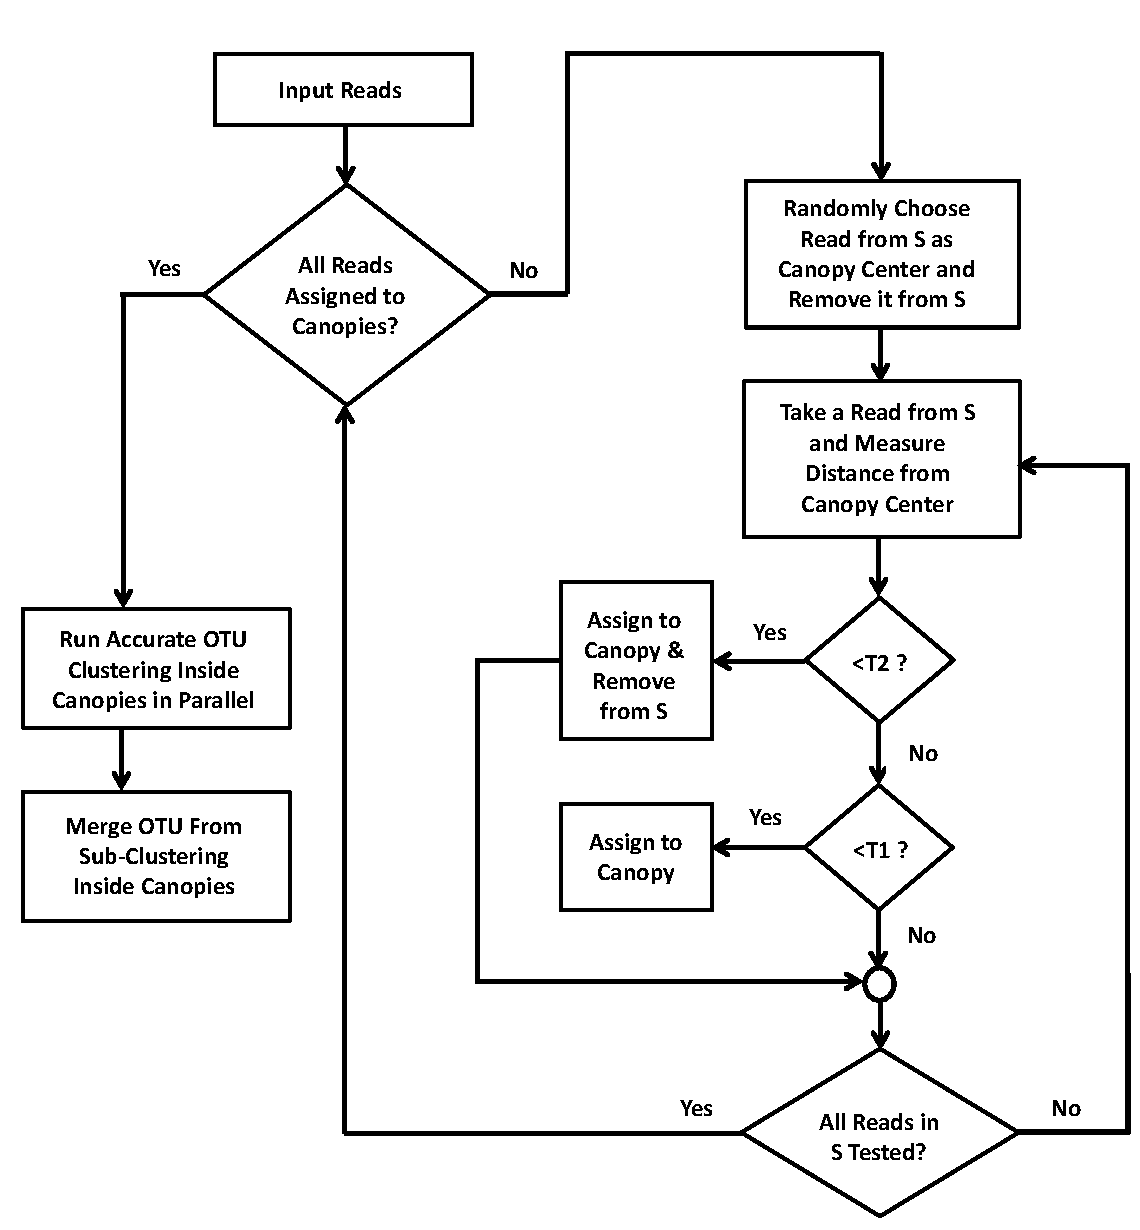
\includegraphics[width=\linewidth,height=10cm]{flowchart.pdf}	
	\caption{Workflow of Canopy Clustering for Large Scale Metagenome Data}
	\label{fig:flowchart}
\end{figure}

In next sections we provide a brief description of Canopy Clustering, Locality Sensitive Hashing, their potential in metagenome data clustering, sub-clustering methods used in this study and two possible methods .  

\subsection{\textbf{Canopy Clustering}}

Canopy Clustering \cite{MARCanopy} is an efficient approximate clustering algorithm often used as preprocessing step for other accurate and expensive clustering methods like the K-means algorithm or the Hierarchical clustering algorithm. It is intended to speed up clustering operations on large data sets, where standard clustering algorithms may be impractical in terms of run time and memory consumptions due to the large number of pairwise distance calculations. For a dataset with $N$ instances, worst case calculations without canopy clustering is $N^2$. After canopy clustering if the number of canopies is $k$ then worst case calculations with canopy clustering is $\sum_{i=1}^{k}(c_i)^2$ where $c_i$ is the number of instances in $i$th canopy. The total difference $g$ in pairwise distance calculations:

\begin{equation}
g=N^2-\sum_{i=1}^{k}(c_i)^2
\end{equation} 

Canopy clustering uses two basic distance thresholds namely \textit{soft} threshold $T1$ and \textit{tight} threshold $T2$. If data point $p_1$ is within the soft distance threshold $T1$ with another data point $p_2$ then $p_1$ will reside in same canopy as $p_2$ but $p_1$ may belong to other canopies assuming that it has only met soft threshold and best match is yet to be found. Thus one data point may belong to multiple canopies in Canopy clustering. On the other hand if data point $p_1$ is within the tight distance threshold $T2$ with another data point $p_2$ then canopy clustering assigns $p_1$ to the same canopy as $p_2$ and stops assigning $p_1$ to any other canopy assuming that tight threshold has been met and best canopy assignment for $p_1$ has been found. In this case $p_1$ will not be repeated in other canopies. Canopy centroids are selected randomly. Then all other data points are tested for canopy assignment based on $T1$ and $T2$. New canopies are selected until all data points are assigned to canopies. A fast approximation based on Locality Sensitive Hashing (LSH) will be used for Canopy membership identification.


\subsection{\textbf{Locality Sensitive Hashing}}

Canopies are intended to reduce pairwise distance calculations since only distances inside canopies are calculated during sub-clustering inside canopies. But Canopy clustering itself should be faster which requires a fast and approximate distance measure only for Canopy assignments. Locality Sensitive Hashing (LSH) \cite{MARLshRef2} is an algorithm for solving the approximate or exact Near Neighbor Search in high dimensional spaces. LSH reduces data dimensionality by randomly projecting data points to low dimensional bit signatures \cite{MARLshRef4}. It also provides approximate measure for fast pairwise distance calculations. LSH has been used for fast comparison between points in very high dimensional space \cite{MARLshRef3}. These characteristics make LSH appropriate for dimensionality reduction and relatively accurate distance measure for Canopy clustering in metagenome data.

In this study we have chosen a random projection based hashing function that projects a $d$ dimensional data point into a $n$ dimensional bit representation where $n<d$. The intuition behind choosing $n<d$ is to reduce dimension of data. Given a random projection $v'$ of size $1 \times d$ and a data vector $a$ of size $1 \times d$, the dot product between them provides a scalar value. Sign of this scalar value represents which side of the random hyperplane does the data point exist. This information can be represented with a single bit. This way a single data point can be represented with limited number of bits. Hamming distance between these binary representations indicates \textit{disagreements} between two data points.

\subsection{\textbf{Sub-Clustering Inside Canopies}}
\label{sub-cluster}
We have used three recent and popular sequence clustering methods as the expensive clustering measure inside canopies in this study. UCLUST \cite{MARuclust}, SUMACLUST \cite{MARSumaclust} and SWARM \cite{MARSwarm} were used for sub-clustering canopies. 

\subsubsection{\textit{UCLUST}}
It is a closed-source software and provides very limited documentations\footnote{http://www.drive5.com/uclust/uclust\_userguide\_1\_1\_579.pdf}. The 32 bit version of UCLUST executable is available for academic usage. But the 64-bit versions which is necessary to handle large datasets, require expensive license. UCLUST follows a greedy process and creates \textit{seeds} of sequences which generate clusters based on percent identity.

\subsubsection{\textit{SUMACLUST}}
An open-source software. It follows similar approach as UCLUST. Based on greedy strategy SUMACLUST incrementally constructs clusters by comparing an abundance-ordered list of input sequences against the representative set of already-chosen sequences. Initially this list is empty.

\subsubsection{\textit{SWARM}}
SWARM uses exhaustive single-linkage clustering based on optimal sequence alignment. Sequences that are less than a certain distance from any other other sequence in the cluster are clustered together. SWARM attempts to reduce the impact of clustering parameters on the resulting OTUs by avoiding arbitrary global clustering thresholds and input sequence ordering dependence. At first SWARM builds an initial set of OTUs is constructed by iteratively agglomerating similar amplicons. Then amplicon abundance values are used to reveal OTUs’ internal structures and to break them into sub-OTUs.

\subsubsection{\textit{Minimum Spanning Tree (MST)}}
To evaluate Canopy as a standalone clustering method along with UCLUST, SUMACLUST and SWARM, we used Minimum Spanning Tree (MST) based clustering method as an accurate and expensive clustering inside canopies. Minimum Spanning Tree (MST) produces a connected spanning tree of undirected graph. It connects all vertices together such that the total weight of edges remains minimum. This property has been used for clustering \cite{MARMstCluster}\cite{MARMstClustering2}\cite{MARMstClustering3}. We represented edges with Locality Sensitive Hashing based distances. Then edges with highest distances were removed from MST to generate OTUs.

\subsection{\textbf{Merging results from Canopies}}

The final step of our proposed framework is to merge the clustered outputs from each canopy provided by more accurate and expensive clustering methods. According to Canopy cluster algorithm a single data point may belong to multiple canopies as long as the soft threshold is met. As a result same or very similar OTUs will be generated from multiple canopies. This scenario is depicted in Figure \ref{fig:merge}. The dashed circles titled OTU-A, B, C and D represent \textit{potential OTUs}. Soild outer circles represent canopies titled Canopy-1, 2 and 3. Smaller triangles, stars, hexagons and rectangles represent sequence reads in metagenome data. OTU-A and C are shared by Canopy-1 and 2. OTU-B and D are shared by Canopy-2 and 3. Since data is already clustered and reduced significantly, this step is relatively faster. Because of this repetitions another final clustering on resulting OTUs is required which will remove repetitions in OTU. We are proposing two solutions to this scenario.

\subsubsection{\textit{Merging with Greedy Clustering Algorithm}}
We have chosen UCLUST for merging step since UCLUST is one of the fastest greedy sequence clustering methods. We chose 90\% identity threshold for UCLUST in this step. Other sequence clustering algorithm can also be applied in this step. Since number of sequences is already reduced by Canopy and accurate clustering, this merging step is very fast. Greedy clustering methods like UCLUST always converges to local minima. Thus this approach does not require number of OTUs as prior. 

\subsubsection{\textit{Merging with Minimum Spanning Tree}}
\label{MST}
We developed a Minimum Spanning Tree and Locality Sensitive Hashing (LSH) distance based metagenome sequence clustering method to be used in merging step as well as inside Canopies for accurate clustering. A brief description of MST based clustering is given in Section \ref{sub-cluster}. Unlike merging with greedy clustering methods, this approach requires number of edges to remove as prior which indicates the number of OTUs.    

\begin{figure}
	\centering
	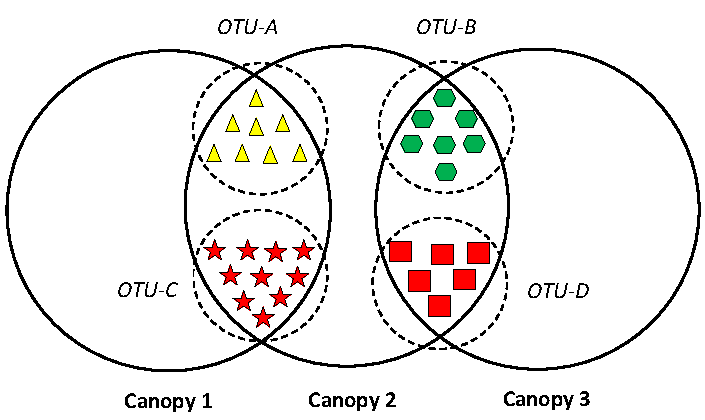
\includegraphics[width=\linewidth,height=4.8cm]{merge.pdf}	
	\caption{Same OTUs Occurring in Multiple Canopies}
	\label{fig:merge}
\end{figure}  
In the following Sections UCLUST, SUMACLUST, SWARM and MST with Canopy clustering approach are represented as CC$_{UCLUST}$, CC$_{SUMACLUST}$, CC$_{SWARM}$ and CC$_{MST}$ respectively where the term CC stands for Canopy Clustering. 

\section{Experimental Evaluation}
\begin{table*}[tb] 
\centering 
\caption{\textbf{Dataset Statistics}} \label{table:finaltabledataset} 
\begin{tabular}{|l| c c c c c c|} 
\hline
\multicolumn{1}{|c|}{{\bf{Datasets}}} & \multicolumn{1}{c}{{\bf{Type}}} & {\bf{Reference}} & {\bf{\# of Reads}} & {\bf{\# of Samples}} & {\bf{Read Length}} & {\bf{Platform}}\\
\hline
{Bokulich$_2$} & Mock & \cite{MARmockDatasetRef} & 6,938,836 & 4 & 189--251 & HiSeq\\
{Bokulich$_3$} & Mock & \cite{MARmockDatasetRef} & 3,594,237 & 4 & 114--151 & HiSeq\\
{Bokulich$_6$} & Mock & \cite{MARmockDatasetRef} & 250,903 & 1 & 114--150 & HiSeq\\
{Canadian Soil} & Genuine & \cite{MARcanadianSoil} & 2,966,053 & 13 & 76--10 & HiSeq\\
{Body Sites} & Genuine & \cite{MARbodySites} & 886,630 & 602 & 117--351 & GS FLX\\
{Global Soil} & Genuine & \cite{MARglobalSoil} & 9,252,764 & 57 & 119--151 & HiSeq\\
\hline
\end{tabular}
\end{table*} 

\subsection{\textbf{Dataset Description}}

%HR EDITS 

To evaluate the performance of our proposed we have used previously published synthetic and real world sequence benchmarks. All of these datasets have been used in previous studies \cite{MARmockDatasetRef} \cite{MARopenDeNovo}. The performance of different open source sequence clustering methods were assessed and compared in a study by Kopylova et. al. \cite{MARopenDeNovo} using these specific datasets. As such, in this paper we use the same benchmarks as done in the prior study. These datasets are publicly available \footnote{https://github.com/ekopylova/otu-clustering}. We used  three synthetic 16S rRNA gene mock community datasets (Bokulich$_2$, Bokulich$_3$, and Bokulich$_6$) from Bokulich et. al. \cite{MARmockDatasetRef} and three real data sets: a 16S rRNA gene soil data set (Canadian Soil) \cite{MARcanadianSoil}, a 16S rRNA gene human data set (Body Sites) \cite{MARbodySites} and 18S rRNA gene soil data set (Global Soil) \cite{MARglobalSoil}. Key statistics and relevant information regarding these datasets are presented in Table \ref{table:finaltabledataset}. 

\textbf{Synthetic Datasets:}

\subsubsection{\textit{Bokulich$_2$}}
This dataset was prepared using the 
Illumina TruSeq v2 paired--end library
preparation kit. It is a simulated 16S rRNA gene 
microbial community data set.
This 
dataset contains 19 taxonomic Families, 19 Genera, 22 Species 
and 22 Strains in total. This dataset can be 
found in the QIIME database (identifier 1685).

\subsubsection{\textit{Bokulich$_3$}}
Similar to Bokulich$_2$ except that it was 
prepared with the 
TruSeq v1 paired-end library kit at 
Illumina Cambridge and is  also available in the 
QIIME database (identifier 1686).

\subsubsection{\textit{Bokulich$_6$}}
This  16S rRNA dataset 
was sequenced at Washington University School of Medicine and 
contains evenly distributed microbial communities. This 
dataset contains 13 taxonomic 
Families, 23 Genera, 44 Species and 48 Strains in total.
%
All these datasets from Bokulich et al.\cite{MARmockDatasetRef} are 
available at QIIME database\footnote{http://qiime.org/home\_static/dataFiles.html} under their respective ID's. Since, these are simulated 
datasets the taxonomic profile of microbial organisms within them 
are known.

\textbf{Real World Datasets:}

\subsubsection{Canadian Soil}
The Canadian Soil dataset\footnote{http://www.cm2bl.org/} contains 
genomic data of soil spanning from Arctic 
Tundra to Agricultural soil suitable for different 
agricultural products.  %etc. in different regions of Canada.

\subsubsection{Body Sites}
This dataset contains composition of 
bacterial communities from up to 27 different 
body sites in healthy adults. A collection of 602 samples acquired from different body sites of human subjects are provided with meta-data.

\subsubsection{Global Soil}
The global soil data was taken from Ramirez et al. \cite{MARglobalSoil} which is a study of the below-ground diversity in New York City's Central Park. 


\subsection{\textbf{Evaluation Metrics}}

We assess the performance of our proposed approach using 
the following types of commonly used metrics that are used 
for the assessment of (i) outputs from clustering algorithms, (ii) biodiversity
within metagenomic samples and (iii) computational run time. 


\subsubsection{\textit{Faith’s phylogenetic diversity metric (PD)}}
Faith’s phylogenetic diversity \cite{MARfaith1992conservation} combines all 
the branch lengths of phylogenetic tree as a measure of diversity. So, if a new 
OTU (cluster)  is found and it is closely related to another OTU in the sample, it will contribute to 
a small increase to the PD score. However, if a new OTU is found and is 
from a different lineage than anything else in the sample, it will contribute to a large 
increase in the PD score.

\subsubsection{\textit{Shannon Entropy}}

Shannon-Wiener diversity index is defined as:

\begin{equation}
H={-} \sum_{i=1}^{s} \left( p_i\log_2p_i \right)
\end{equation}

where s is the number of OTUs and $p_i$ is the proportion of the community represented by OTU $i$. The Shannon index increases as both the richness and evenness of the community increase. The fact that the index incorporates both components of biodiversity can be seen as both a strength and a weakness. It is a strength because it provides a simple summary, but it is a weakness because it makes it difficult to compare communities that differ greatly in richness.


\subsubsection{\textit{Simpson's Index}}
Simpson’s index is defined as ${1-dominance}$ or

\begin{equation}
1 - \sum p_i^2
\end{equation}

where where $p_i$ is the proportion of the community represented by OTU $i$. Simpsonʼs index is based on the probability that any two individuals drawn at random from an infinitely large community belong to the same species. It measures \textit{evenness} of the community from 0 to 1. Higher value of this index implies higher similarity and relatively lower diversity of microorganisms within a sample.


\subsubsection{\textit{F-measure}}
In case of synthetic datasets, false-positive (FP; taxonomy/OTU string 
exists in observed but not expected), false-negative
(FN; taxonomy/OTU exists in expected but not observed), and 
true-positive (TP; taxonomy/OTU exists in both observed and expected) measures were computed from 
cluster output and the ground truth which is the expected taxonomic composition. The following definitions were used:

\begin{equation}
precision = \frac{TP}{(TP + FP)}
\end{equation}

\begin{equation}
recall = \frac{TP}{(TP + FN)}
\end{equation}

\begin{equation}
F Score = \frac{2 \times precision \times recall}{(precision + recall)}
\end{equation}

\subsubsection{\textit{Pearson Coefficient Correlation ($\rho$-value)}}
After getting Operational Taxonomic Units (OTU) from a clustering method we create a taxonomic profile at the Genus level. Pearson’s correlation coefficient was computed to measure the relatedness of taxonomic assignment between a pair of tools. Values can range between -1 and 1, with -1 indicating a negative correlation, 0 indicating no correlation, and 1 indicating a positive correlation or strong relationship.


\subsection{\textbf{Parameter Setting}}

For kmers, the value of parameter K was set to 4. There are 4 possible nucleotide representatives (A,C,G and T) and the total number of features became $4^4=256$. This way we were able to convert the string representation into numeric. For Locality Sensitive Hashing the number of Hyperplanes (parameter $d$) was set to 150. We wanted to reduce the number of features while maintaining a relatively accurate distance approximation. So value of $d$ was chosen to be less than 256. For performance analysis and comparison we have chosen $T1=0.45$ and $T2=0.34$.         

We performed all the experiments on computers with Intel 5th generation Core i7 2.70GHz 64bit processor with 8 core CPUs and 12GB memory. For implementation we used Python 2.7.12 and QIIME \cite{MARQiime} version 1.9.0 - a popular open source Bioinformatics pipeline that combines many metagenome clustering methods including the ones which has been used in this work. One important aspect our proposed approach is parallelism. Each canopy can be clustered in parallel. To take full advantage of today's multi-core CPU based computing systems we utilized Python's \textit{multiprocessing} module instead of \textit{threading} module. According to Python's documentation\footnote{https://docs.python.org/2/library/multiprocessing.html} \textit{multiprocessing} module allows the programmer to fully leverage multiple processors on a given machine by spawning subprocesses instead of threads. After receiving output from all canopy clustering we merged the outputs to make a single clustering results. Some performance metric used in this study like Faith’s Phylogenetic Diversity (PD) metric require sequence alignment. We used PyNast\footnote{http://biocore.github.io/pynast/} \cite{MARPynast} open source sequence aligner for aligning clustered output.    


\section{Results Discussion} 
\label{sec:results}

\subsection{\textbf{Clustering Performance Comparison}}
Table \ref{table:performanceTable} shows the performance of  UCLUST \cite{MARuclust}, 
SUMACLUST \cite{MARSumaclust} and SWARM \cite{MARSwarm} and their corresponding versions with our proposed approach. Table \ref{table:performanceTable} compares F-scores and Pearson Correlation Coefficient ($\rho$). F-scores are only available for synthetic benchmarks since taxanomic profile for them is known as ground truth. But F-scores are not available for real benchmarks as no ground truth is available for them. Correlation values were generated based on taxonomic profiles at Genus level generated from outputs from clustering methods. From Table \ref{table:performanceTable} we can see that F-scores obtained from a clustering method and its corresponding Canopy clustering version are very closer, in some cases better. We got higher F-score for Bokulich$_2$ benchmark from CC$_{SUMACLUST}$. CC$_{UCLUST}$ and CC$_{SWARM}$ provided same F-scores as their respective naive versions for Bokulich$_2$. For Bokulich$_3$ benchmark we observed higher F-scores for all LSH based Canopy clustering methods. Finally for Bokulich$_6$ benchmark F-scores of UCLUST and SWARM were improved comparing to respective naive versions.

For all benchmarks we got very strong correlations between taxonomic profiles at genus level from UCLUST, SUMACLUST, SWARM and their respective LSH based Canopy counterparts. The highest correlation was observed for Bokulich$_6$ benchmark between UCLUST and CC$_{UCLUST}$ with 0.9831 and the lowest was observed for Canadian Soil metagenome data between SUMACLUST and CC$_{SUMACLUST}$ with 0.7581. From observed F-scores and correlation values we can say that running a sequence clustering method with our proposed LSH based Canopy cluster framework can bring similar or better results. Next we will discuss about Runtime Comparisons. CC$_{MST}$ provided relatively similar F-scores and high $\rho$ values indicating strong correlations of taxonomic outcomes with other methods. 

\subsection{\textbf{Runtime Comparison}} Table \ref{table:Runtime} shows the runtime in minutes of UCLUST, SUMACLUST, SWARM, MST and their respective versions with our proposed Canopy clustering pipeline. Time information in Table \ref{table:Runtime} was recorded while populating performance metric values for Table \ref{table:performanceTable} for the parameter setting mentioned in Experimental Details section. Improving runtime while maintaining similar or better clustering results was one of the major motivations of our proposed approach. We can see from Table \ref{table:Runtime} that CC$_{UCLUST}$ outperforms UCLUST for all datasets. The highest speed up for UCLUST was observed for Bokulich$_2$ dataset where UCLUST was 2.10 times faster with LSH based Canopy than the naive version. For SUMACLUST we can see from Table \ref{table:Runtime} that CC$_{SUMACLUST}$ outperforms naive SUMACLUST in most cases. Major improvement in runtime was observed in large scale real world metagenome datasets specially Canadian Soil and Global Soil datasets. The highest speed-up for SUMACLUST with Canopy clustering was observed to be 7.70x for Global Soil dataset.

We can see a similar footprints for CC$_{SWARM}$ and CC$_{MST}$ from Table \ref{table:Runtime}. The highest speedup in runtime for SWARM and MST with Canopy clustering was observed to be 4.79x and 2.01x respectively for Global Soil dataset which is the largest dataset used in this study. From these observations we can conclude that LSH based Canopy clustering not only reduces the runtime of an expensive clustering method but also scales well and performs better for larger benchmark datasets comparing to the smaller ones.   

\subsection{\textbf{Biodiversity Comparison}} Clustering sequences in metagenome data will provide OTUs that represent biodiversity contained in the samples from which data is collected. Hence we also need to compare the biodiversity represented by OTUs from naive methods and their respective Canopy clustering variations used in this study. Table \ref{table:bioDiversityTable} shows Faith’s phylogenetic diversity metric (PD), Shannon and Simpson index after clustering with different methods. These metrics are some of the popular Alpha Diversity metrics meaning that they measure species diversity in sites or habitats at a local scale. These metric values are generated per sample basis. Table \ref{table:bioDiversityTable} shows ranges of metric values in $[minimum-maximum]$ format provided by methods with and without Canopy clustering. Any sample of a dataset will take value from this range. These ranges may not be same since OTUs vary over clustering methods. But they should be similar. We can see from Table \ref{table:bioDiversityTable} that Canopy clustering based methods produce similar ranges of values as their naive counterparts. No significant changes in diversity metric values were observed which indicates that Canopy based approaches reproduce similar biodiversity while reducing runtime.          


\begin{table*}[t]
	\centering 
	\caption{\textbf{Performance Comparison [$F$-Score and Pearson Correlation Coefficient ($\rho$)]}} 
	\label{table:performanceTable}
	
	\scalebox{0.95}{
		
		\begin{tabular}{|l|c c c c| c c c|}
			
			\hline
			
			\textbf{Methods} & \textbf{Comparison Metric} & \multicolumn{6}{c|}{\textbf{Datasets}}\\
			
			\cline{3-8}
			
			& & \multicolumn{3}{c|}{\textit{Synthetic}} & \multicolumn{3}{c|}{\textit{Real World}}\\ 
			
			\cline{3-8}
			
			&  & Bokulich$_2$ & Bokulich$_3$ & Bokulich$_6$ & Body Sites & Canadian Soil & Global Soil\\
			
			\hline
			
			\multirow{1}{*}{UCLUST} & $F$-Measure & 0.39 & 0.40 & 0.51 & $N/A$ & $N/A$ & $N/A$\\
			
			\hdashline
			
			\multirow{2}{*}{CC$_{UCLUST}$} & $F$-Measure & \textit{\textbf{0.39}} & \textit{\textbf{0.41}} & \textit{\textbf{0.52}} & $N/A$ & $N/A$ & $N/A$\\
			& Correlation ($\rho$) with Respect to UCLUST & \textit{\textbf{0.9831}} & \textit{\textbf{0.9753}} & \textit{\textbf{0.9831}} & \textit{\textbf{0.9682}} & \textit{\textbf{0.8419}} & \textit{\textbf{0.9824}}\\
			
			\hline 
						
			\multirow{1}{*}{SUMACLUST} & $F$-Measure & 0.40 & 0.41 & 0.51 & $N/A$ & $N/A$ & $N/A$\\
						
			\hdashline
			
			\multirow{2}{*}{CC$_{SUMACLUST}$} & $F$-Measure & \textit{\textbf{0.41}} & \textit{\textbf{0.42}} & \textit{\textbf{0.51}} & $N/A$ & $N/A$ & $N/A$\\
			& Correlation ($\rho$) with Respect to SUMACLUST & \textit{\textbf{0.9709}} & \textit{\textbf{0.9813}} & \textit{\textbf{0.9538}} & \textit{\textbf{0.9518}} & \textit{\textbf{0.7643}} & \textit{\textbf{0.8714}}\\ 
			
			\hline
			
			\multirow{1}{*}{SWARM} & $F$-Measure & 0.46 & 0.48 & 0.55 & $N/A$ & $N/A$ & $N/A$\\
						
			\hdashline
			
			\multirow{2}{*}{CC$_{SWARM}$} & $F$-Measure & \textit{\textbf{0.46}} & \textit{\textbf{0.49}} & \textit{\textbf{0.56}} & $N/A$ & $N/A$ & $N/A$\\
			& Correlation ($\rho$) with Respect to SWARM & \textit{\textbf{0.9817}} & \textit{\textbf{0.97861}} & \textit{\textbf{0.9251}} & \textit{\textbf{0.9648}} & \textit{\textbf{0.7581}} & \textit{\textbf{0.9143}}\\
			
			\hline
			
			\multirow{4}{*}{CC$_{MST}$} & $F$-Measure & 0.41 & 0.42 & 0.52 & $N/A$ & $N/A$ & $N/A$\\
			& Correlation ($\rho$) with respect to UCLUST & 0.7461 & 0.8143 & 0.8272 & 0.7417 & 0.6935 & 0.7974 \\ & Correlation ($\rho$) with respect to SUMACLUST & 0.7182 & 0.6903 & 0.8613 & 0.8293 & 0.6791 & 0.8213 \\  & Correlation ($\rho$) with respect to SWARM & 0.7914 & 0.7352 & 0.8904 & 0.7619 & 0.7372 & 0.8502  \\
			
			\hline
			
		\end{tabular}
	}
	\small
	\begin{tablenotes}
		\item Table shows values of $F$-measures and Pearson Correlation Coefficient ($\rho$-value) of UCLUST, SUMACLUST, SWARM and their respective versions with Canopy clustering. $F$-measures is only available for synthetic datasets but not for real world datasets since no ground truths like known taxonomic profiles are available for them. $\rho$-value was calculated based on the taxonomy profiles at Genus level generated from clustered OTUs provided by a method and it's corresponding LSH based Canopy counterpart. Higher $F$-measures reflect better clustering by adhering to ground truth. Higher $\rho$-values reflect stronger correlation between taxonomic profiles.        
	\end{tablenotes}
	
\end{table*} 


\begin{table*}
	\centering
	\caption{\textbf{Runtime Comparison (in minutes)}} 
	\label{table:Runtime}
	\scalebox{0.56}{
		\begin{tabular}{|c c c|c c c c|c c c c|c c c c|c c c c|} 
			
			\hline
			
			\multicolumn{3}{|c|}{\textbf{Datasets}} & \multicolumn{16}{c|}{\textbf{Methods}}\\
			%\cline{3-9}
			
			\hline
			
			\multirow{3}{*}{Type} & \multirow{3}{*}{Title} & \multirow{3}{*}{\# of Reads} & \multirow{3}{*}{UCLUST} & & \multirow{1}{*}{UCLUST} & \multirow{3}{*}{Speed Up} & \multirow{3}{*}{SUMACLUST} & & \multirow{1}{*}{SUMACLUST} & \multirow{3}{*}{Speed Up} & \multirow{3}{*}{SWARM} & & \multirow{1}{*}{SWARM} & \multirow{3}{*}{Speed Up} & \multirow{3}{*}{MST} & & \multirow{1}{*}{MST} & \multirow{3}{*}{Speed Up}\\
			
			& & & & Canopy Only & with & & & Canopy Only & with & & & Canopy Only & with & & & Canopy Only & with & \\
			
			& & & & & Canopy & & & & Canopy & & & & Canopy & & & & Canopy & \\ 
			
			\hline
			
			\multirow{3}{*}{\textit{Synthetic}} & Bokulich$_2$ & 6,938,836 & 12.71 & 4.81 & \textit{\textbf{6.03}} & \textit{\textbf{2.10x}} & 87.53 & 5.73 & \textit{\textbf{33.03}} & \textit{\textbf{2.65x}} & 128.12 & 5.29 & \textit{\textbf{37.87}} & \textit{\textbf{3.38x}} & 564.60 & 5.62 & \textit{\textbf{294.36}} & \textit{\textbf{1.91x}}\\       
			& Bokulich$_3$ & 3,594,237 & 8.91 & 2.91 & \textit{\textbf{4.89}} & \textit{\textbf{1.82x}} & 11.73 & 3.05 & \textit{\textbf{7.89}} & \textit{\textbf{1.48x}} & 9.10 & 2.98 & \textit{\textbf{6.93}} & \textit{\textbf{1.31x}} & 369.7 & 2.94 & \textit{\textbf{204.61}} & \textit{\textbf{1.80x}}\\       
			& Bokulich$_6$ & 250,903 & 1.21 & 0.49 &  \textit{\textbf{1.08}} & \textit{\textbf{1.12x}} & \textit{\textbf{1.28}} & 0.52 & 1.34 & 0.96 & 1.97 & 0.51 & \textit{\textbf{1.29}} & \textit{\textbf{1.53x}} & 252.81 & 0.62 & \textit{\textbf{146.41}} & \textit{\textbf{1.73x}}\\ 
			
			\hline
			
			\multirow{3}{*}{\textit{Real World}} & Body Sites & 886,630 & 2.12 & 1.03 & \textit{\textbf{1.51}} & \textit{\textbf{1.40x}} & 15.42 & 1.09 & \textit{\textbf{7.88}} & \textit{\textbf{1.95x}} & 3.64 & 0.98 & \textit{\textbf{1.71}} & \textit{\textbf{2.13x}} & 307.2 & 1.10 & \textit{\textbf{174.27}} & \textit{\textbf{1.76x}}\\
			& Canadian Soil & 2,966,053 & 9.55 & 2.18 & \textit{\textbf{5.91}} & \textit{\textbf{1.62x}} & 363.96 & 2.91 & \textit{\textbf{81.18}} & \textit{\textbf{4.48x}} & 97.50 & 3.11 & \textit{\textbf{32.16}} & \textit{\textbf{3.03x}}  & 472.43 & 2.43 & \textit{\textbf{254.91}} & \textit{\textbf{1.85x}}\\
			& Global Soil & 9,252,764 & 72.47 & 21.38 &  \textit{\textbf{43.53}} & \textit{\textbf{1.67x}} & 510.92 & 20.82 & \textit{\textbf{66.27}} & \textit{\textbf{7.70x}} & 269.07 & 21.17 &  \textit{\textbf{56.14}} & \textit{\textbf{4.79x}} & 988.93 & 21.43 & \textit{\textbf{464.29}} & \textit{\textbf{2.13x}}\\
			
			\hline 
			
		\end{tabular}
	}
\end{table*}
          

\begin{table*}[t]
	\centering 
	\caption{\textbf{Biodiversity Comparison [Faith’s phylogenetic diversity metric (PD), Shannon and Simpson]}} 
	\label{table:bioDiversityTable}
	
	\scalebox{0.88}{
		
		\begin{tabular}{|c|c c c c| c c c|}
			
			\hline
			
			\textbf{Methods} & \textbf{Comparison Metric} & \multicolumn{6}{c|}{\textbf{Datasets}}\\
			
			\cline{3-8}
			
			& & \multicolumn{3}{c|}{\textit{Synthetic}} & \multicolumn{3}{c|}{\textit{Real World}}\\ 
			
			\cline{3-8}
			
			&  & Bokulich$_2$ & Bokulich$_3$ & Bokulich$_6$ & Body Sites & Canadian Soil & Global Soil\\
			
			\hline
			
			\multirow{3}{*}{UCLUST} & PD Range & $\left[171.95-221.85\right]$ & $\left[186.90-212.84\right]$ & $\left[104.51-104.51\right]$ & $\left[1.46-46.79\right]$ & $\left[0.30-1352.73\right]$ & $\left[2.98-3.29\right]$\\ 
			& Shannon Range & $\left[2.52-3.51\right]$ & $\left[2.43-3.54\right]$ & $\left[5.87-5.87\right]$ & $\left[0.29-7.67\right]$ & $\left[2.32-10.85\right]$ & $\left[1.84-8.30\right]$\\
			& Simpson Range & $\left[0.55-0.75\right]$ & $\left[0.55-0.76\right]$ & $\left[0.96-0.96\right]$ & $\left[0.049-0.98\right]$ & $\left[0.80-0.99\right]$ & $\left[0.0-0.98\right]$\\
			
			& & & & & & & \\
			
			\multirow{3}{*}{CC$_{UCLUST}$} & PD Range & $\left[164.79-217.72\right]$ & $\left[169.41-198.36\right]$ & $\left[109.33-109.33\right]$ & $\left[2.37-47.13\right]$ & $\left[0.52-1419.31\right]$ & $\left[3.02-3.81\right]$\\
			& Shannon Range & $\left[2.61-3.83\right]$ & $\left[2.92-3.91\right]$ & $\left[6.41-6.41\right]$ & $\left[0.93-7.13\right]$ & $\left[3.26-7.61\right]$ & $\left[3.72-7.38\right]$\\
			& Simpson Range & $\left[0.64-0.87\right]$ & $\left[0.56-0.93\right]$ & $\left[0.96-0.96\right]$ & $\left[0.081-0.99\right]$ & $\left[0.84-0.99\right]$ & $\left[0.21-0.99\right]$\\
			
			\hline
			
			\multirow{3}{*}{SUMACLUST} & PD Range & $\left[106.00-162.78\right]$ & $\left[142.85-174.19\right]$ & $\left[89.22-89.22\right]$ & $\left[0.93-39.47\right]$ & $\left[0.59-1279.29\right]$ & $\left[2.98-3.29\right]$\\
			& Shannon Range & $\left[2.00-3.01\right]$ & $\left[2.19-3.28\right]$ & $\left[5.48-5.48\right]$ & $\left[0.16-7.43\right]$ & $\left[2.32-7.32\right]$ & $\left[1.00-7.89\right]$\\
			& Simpson Range & $\left[0.52-0.73\right]$ & $\left[0.54-0.75\right]$ & $\left[0.95-0.95\right]$ & $\left[0.027-0.98\right]$ & $\left[0.80-0.99\right]$ & $\left[0.40-0.98\right]$\\
			
			& & & & & & & \\
			
			\multirow{3}{*}{CC$_{SUMACLUST}$} & PD Range & $\left[114.96-171.57\right]$ & $\left[147.85-187.91\right]$ & $\left[93.81-93.81\right]$ & $\left[0.86-41.63\right]$ & $\left[0.81-1292.34\right]$ & $\left[1.37-4.89\right]$\\
			& Shannon Range & $\left[2.51-3.94\right]$ & $\left[2.96-4.11\right]$ & $\left[5.94-5.94\right]$ & $\left[1.21-7.13\right]$ & $\left[3.12-7.79\right]$ & $\left[2.17-7.25\right]$\\
			& Simpson Range & $\left[0.68-0.79\right]$ & $\left[0.51-0.74\right]$ & $\left[0.96-0.96\right]$ & $\left[0.06-0.99\right]$ & $\left[0.88-0.99\right]$ & $\left[0.23-0.98\right]$\\
			
			\hline
			
			\multirow{3}{*}{SWARM} & PD Range & $\left[18.37-24.73\right]$ & $\left[17.36-19.81\right]$ & $\left[30.84-30.84\right]$ & $\left[1.44-28.66\right]$ & $\left[0.54-706.57\right]$ & $\left[5.79-6.18\right]$\\ 
			& Shannon Range & $\left[2.98-3.91\right]$ & $\left[2.01-3.04\right]$ & $\left[5.03-5.03\right]$ & $\left[0.28-7.63\right]$ & $\left[1.0-7.79\right]$ & $\left[1.66-7.81\right]$\\
			& Simpson Range & $\left[0.70-0.82\right]$ & $\left[0.53-0.74\right]$ & $\left[0.95-0.95\right]$ & $\left[0.05-0.98\right]$ & $\left[0.50-0.99\right]$ & $\left[0.00-0.99\right]$\\
			
			& & & & & & & \\
			
			\multirow{3}{*}{CC$_{SWARM}$} & PD Range & $\left[19.18-26.87\right]$ & $\left[18.43-22.61\right]$ & $\left[31.48-31.48\right]$ & $\left[2.34-29.97\right]$ & $\left[1.37-748.71\right]$ & $\left[2.34-8.46\right]$\\
			& Shannon Range & $\left[1.66-4.87\right]$ & $\left[1.19-4.13\right]$ & $\left[6.03-6.03\right]$ & $\left[0.89-7.13\right]$ & $\left[2.81-8.06\right]$ & $\left[2.81-7.87\right]$\\
			& Simpson Range & $\left[0.66-0.88\right]$ & $\left[0.41-0.81\right]$ & $\left[0.91-0.91\right]$ & $\left[0.11-0.99\right]$ & $\left[0.74-0.99\right]$ & $\left[0.14-0.99\right]$\\
			
			\hline
			
			\multirow{3}{*}{CC$_{MST}$} & PD Range & $\left[10.43-89.61\right]$ & $\left[12.83-92.41\right]$ & $\left[63.21-63.21\right]$ & $\left[1.46-34.15\right]$ & $\left[2.73-824.62\right]$ & $\left[1.81-5.37\right]$\\ 
			& Shannon Range & $\left[0.96-3.91\right]$ & $\left[1.21-3.16\right]$ & $\left[4.91-4.91\right]$ & $\left[2.02-6.51\right]$ & $\left[2.72-7.83\right]$ & $\left[2.17-6.29\right]$\\
			& Simpson Range & $\left[0.14-0.68\right]$ & $\left[0.32-0.73\right]$ & $\left[0.92-0.92\right]$ & $\left[0.07-0.94\right]$ & $\left[0.58-0.94\right]$ & $\left[0.14-0.98\right]$\\
			
			\hline
			
		\end{tabular}
	}
	\small
	\begin{tablenotes}
		\item Table shows ranges of values for Faith’s Phylogeny Diversity (PD), Shannon and Simpson coefficient over all samples in a dataset in the format $[minimum-maximum]$. Most of these datasets contain multiple samples and Alpha diversity metrics like PD, Shannon and Simpson values are generated for each of these samples separately. Biodiversity metric values changes significantly over samples e.g. diversity from hair samples and teeth cavity are supposedly different. So instead of mean values this Table represents $[minimum-maximum]$  ranges of values a sample can take. Similar ranges reflect similar diversity.      
	\end{tablenotes}
	
\end{table*} 


   
\begin{figure}[t]
	
	\begin{minipage}[t]{0.5\linewidth}
		\subfloat[]{
			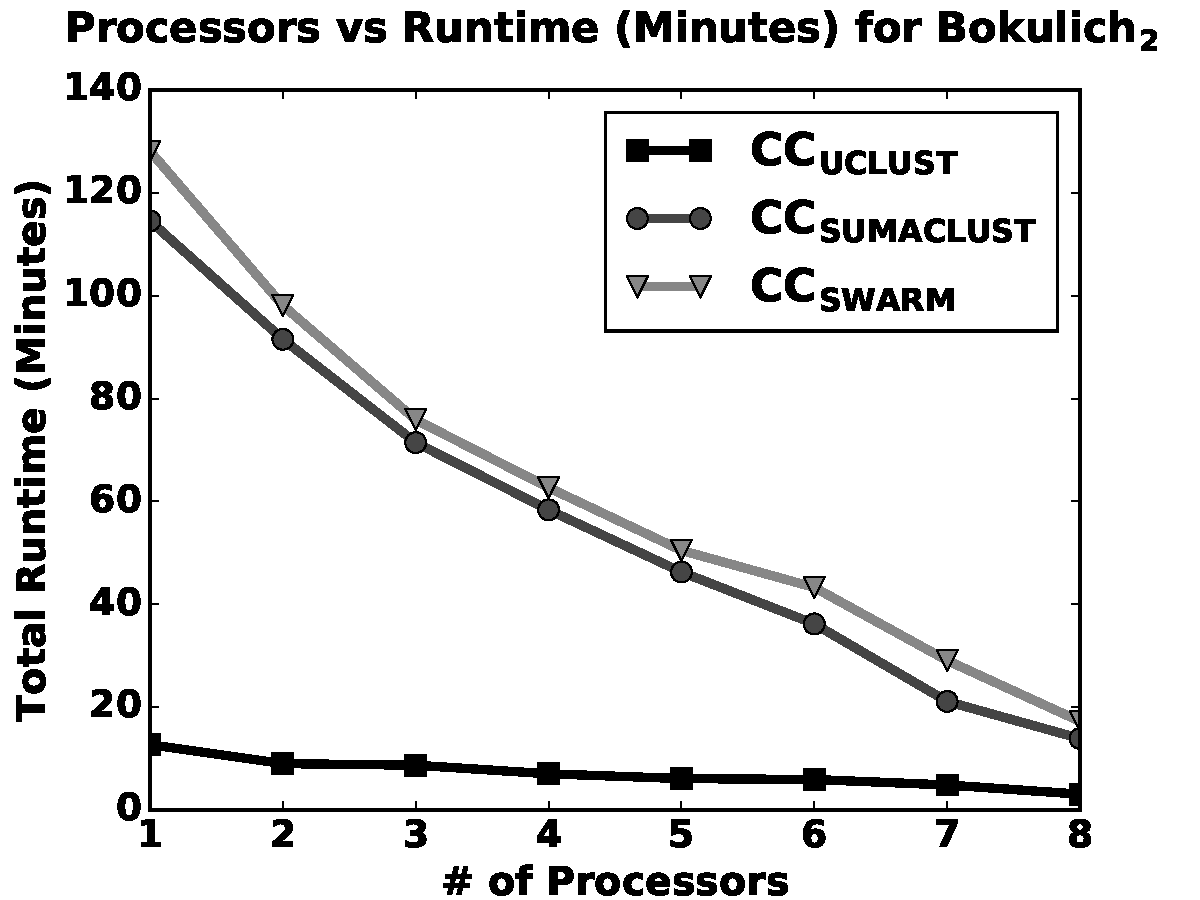
\includegraphics[width=\linewidth]{bokulich_2.pdf}
		\label{fig:bokulich_2}}
	\end{minipage}%
	\hfill%
	\begin{minipage}[t]{0.5\linewidth}
		\subfloat[]{
			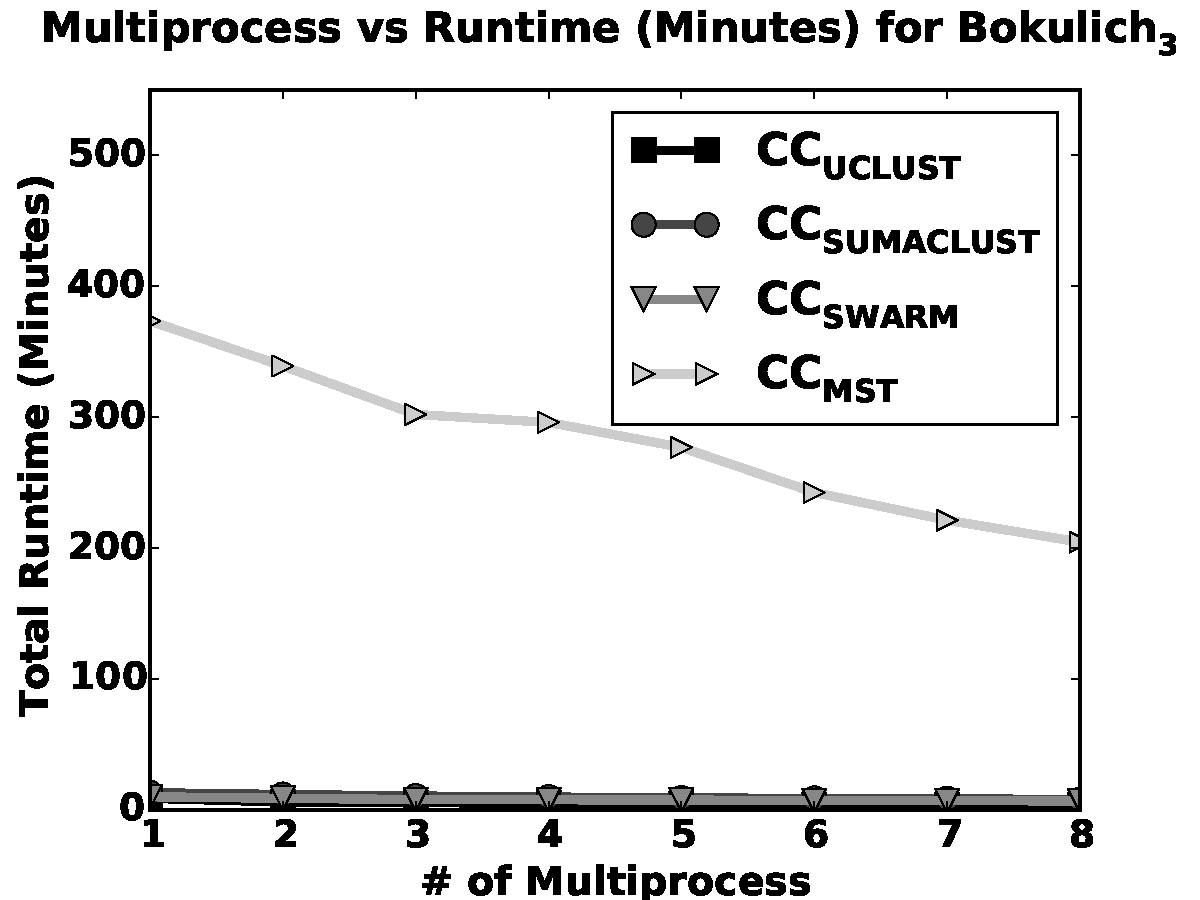
\includegraphics[width=\linewidth]{bokulich_3.pdf}
		\label{fig:bokulich_3}}
	\end{minipage} \\
	
	\begin{minipage}[t]{0.5\linewidth}
		\subfloat[]{
			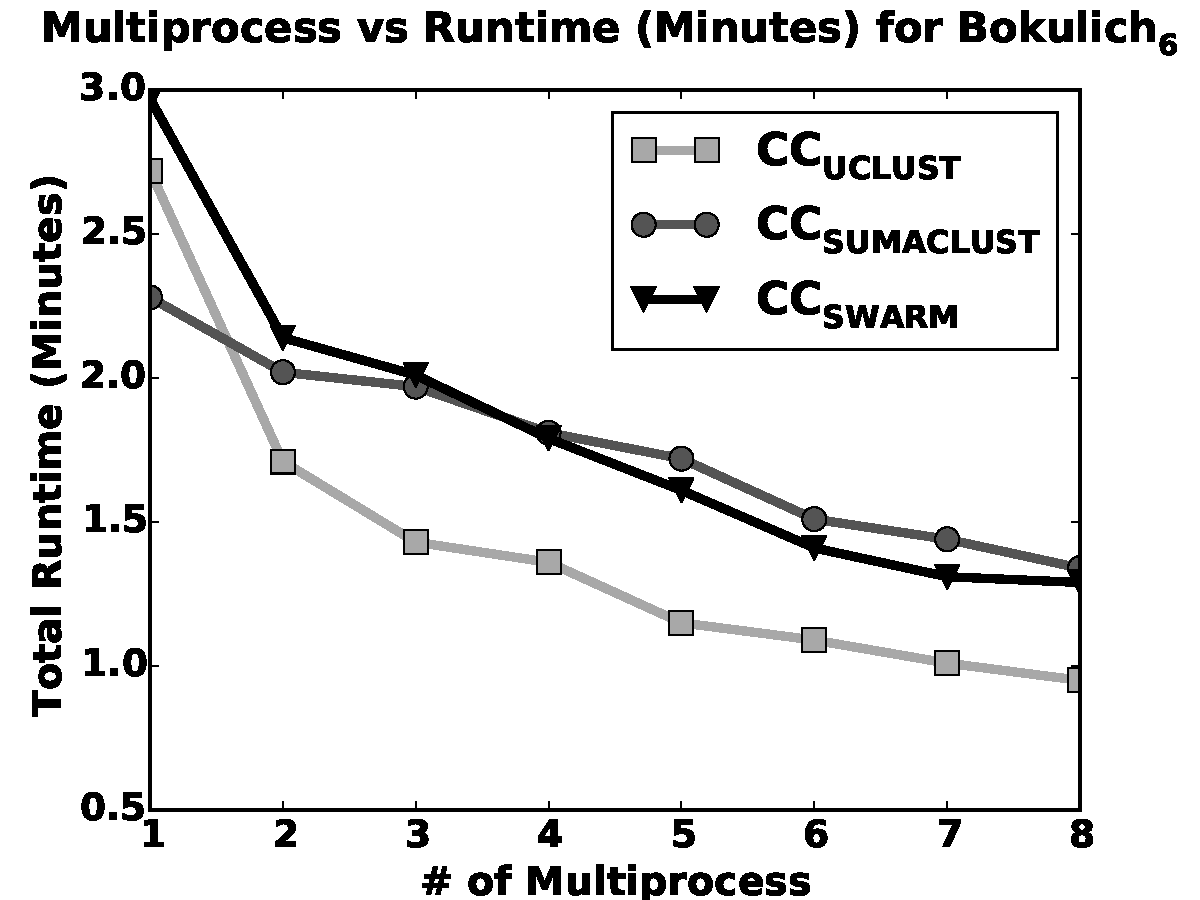
\includegraphics[width=\linewidth]{bokulich_6.pdf}
		\label{fig:bokulich_6}}
	\end{minipage}%
	\hfill%
	\begin{minipage}[t]{0.5\linewidth}
		\subfloat[]{
			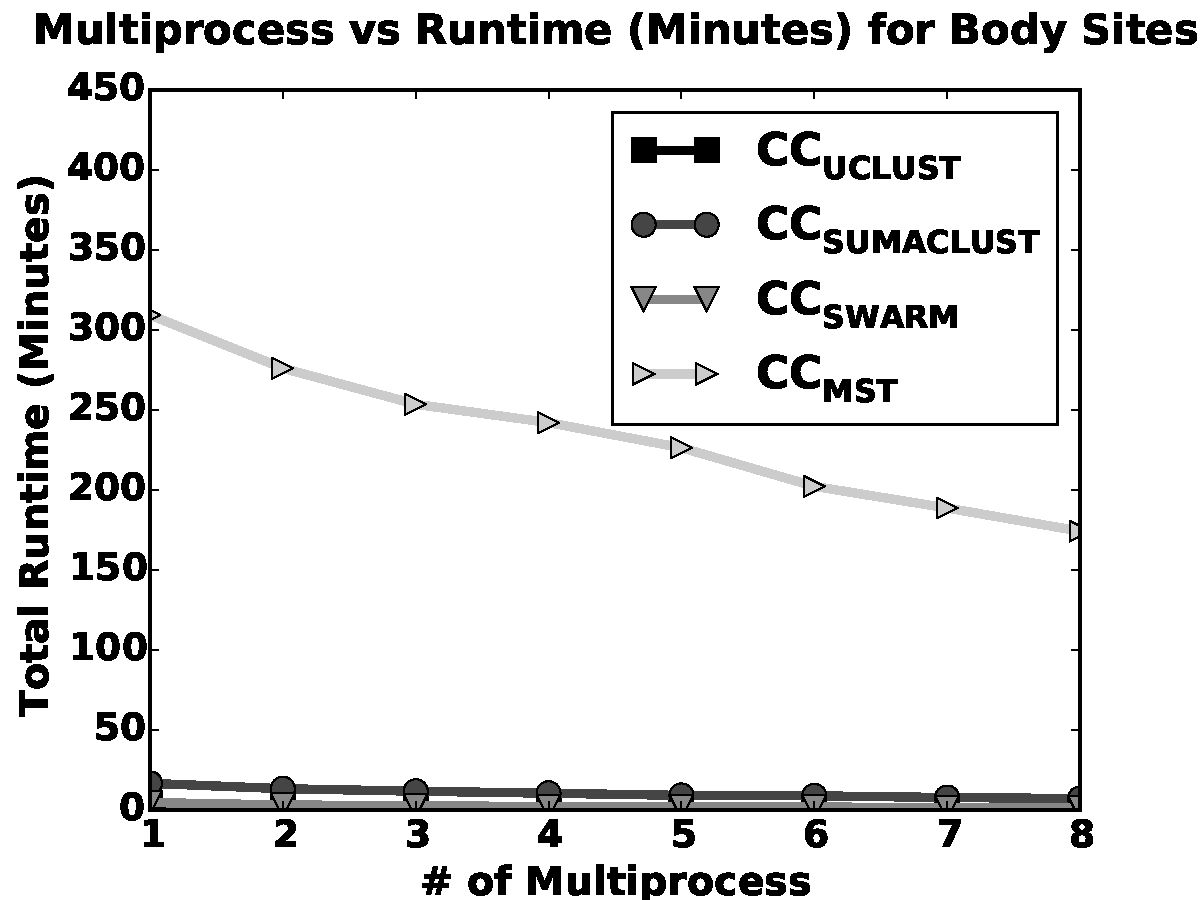
\includegraphics[width=\linewidth]{body_sites.pdf}
		\label{fig:body_sites}}
	\end{minipage} \\
	
	\begin{minipage}[t]{0.5\linewidth}
		\subfloat[]{
			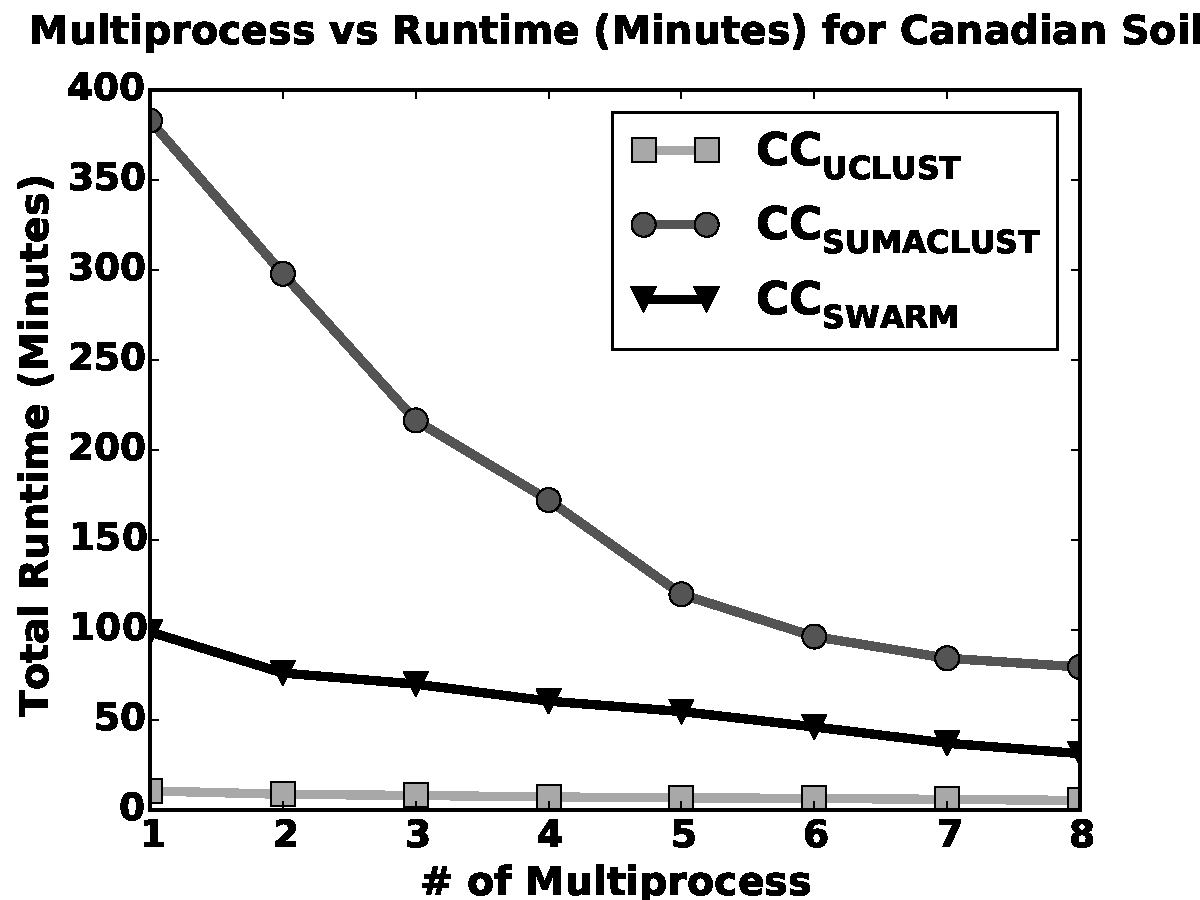
\includegraphics[width=\linewidth]{canadian_soil.pdf}
			\label{fig:canadian_soil}}
	\end{minipage}%
	\hfill%
	\begin{minipage}[t]{0.5\linewidth}
		\subfloat[]{
			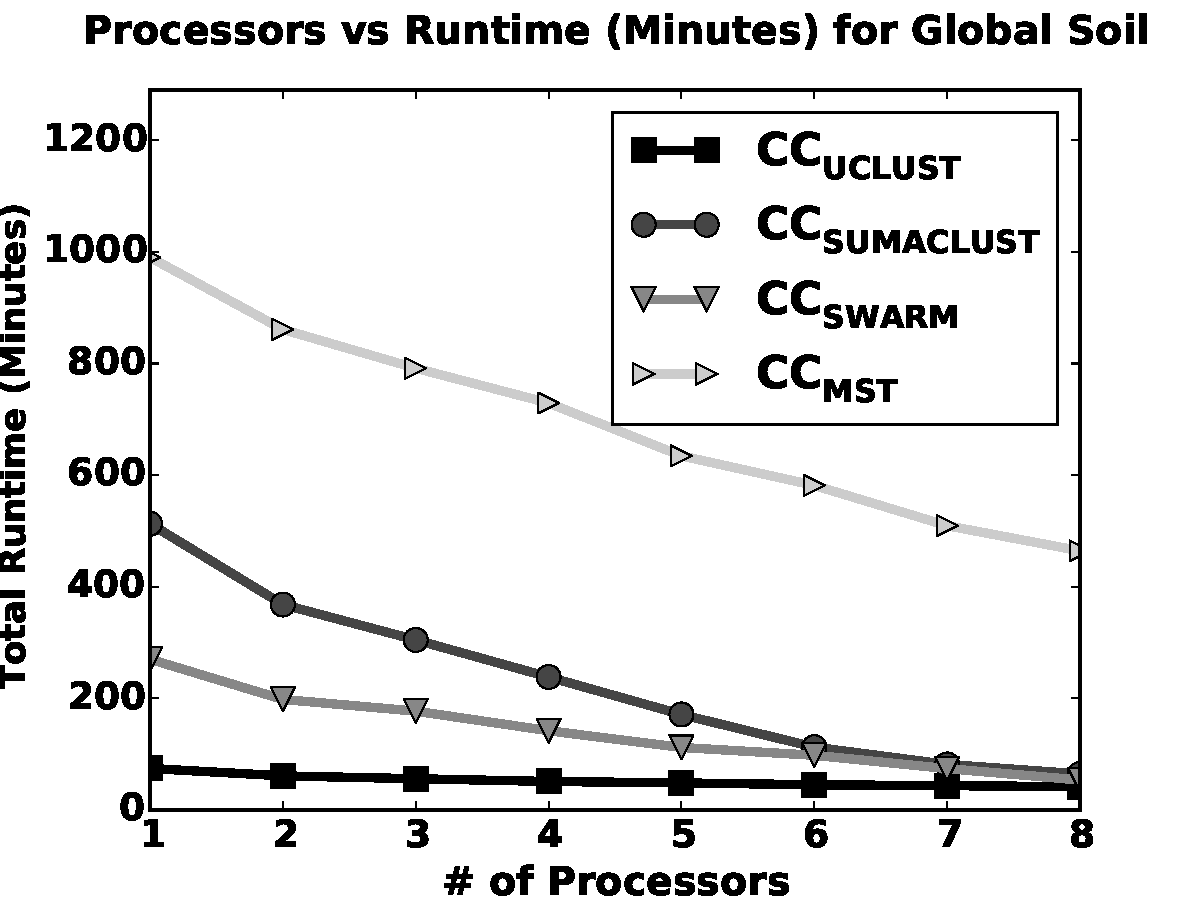
\includegraphics[width=\linewidth]{global_soil.pdf}
			\label{fig:global_soil}}
	\end{minipage}
	
	\caption{Runtime comparison of Canopy clustering framework with UCLUST, SUMACLUST and SWARM on Bokulich$_2$, Bokulich$_3$, Bokulich$_6$, Body Sites, Canadian Soil and GLobal Soil datasets.}

\end{figure}


\begin{figure}[t]	
	\begin{minipage}[t]{0.5\linewidth}
		\subfloat[]{
			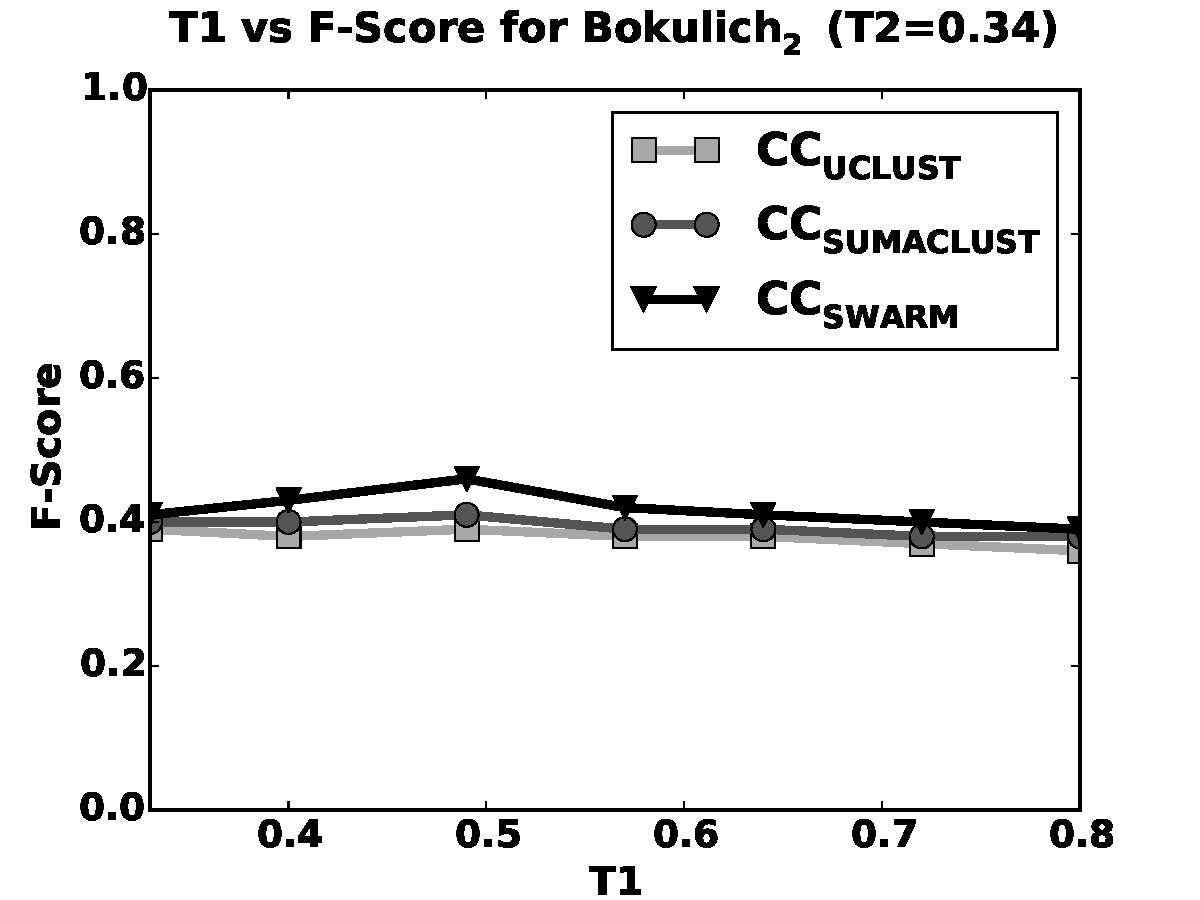
\includegraphics[width=\linewidth]{bokulich_2_T1.pdf}
			\label{fig:bokulich_2_T1}}
	\end{minipage}%
	\hfill%
	\begin{minipage}[t]{0.5\linewidth}
		\subfloat[]{
			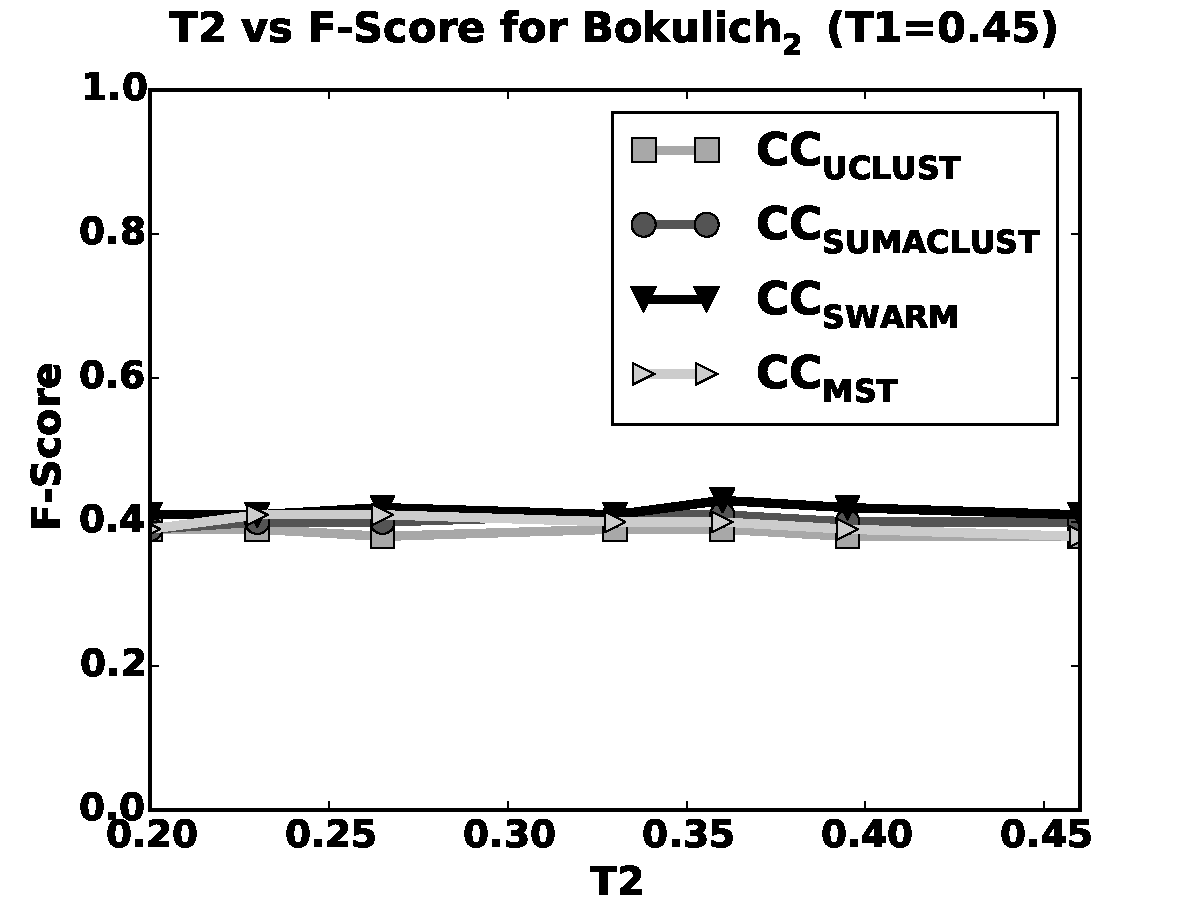
\includegraphics[width=\linewidth]{bokulich_2_T2.pdf}
			\label{fig:bokulich_2_T2}}
	\end{minipage}
	\caption{ \ref{fig:bokulich_2_T1} and \ref{fig:bokulich_2_T2} show effect of varying $T1$ and $T2$ on $F$-scores for the largest synthetic dataset Bokulich$_2$ }	
\end{figure}


\subsection{\textbf{Effect of Varying Number of Multi-processes}}
Figure \ref{fig:bokulich_2}-\ref{fig:global_soil} shows how the number of multiprocess can affect runtime of CC$_{UCLUST}$, CC$_{SUMACLUST}$ and CC$_{SWARM}$ on six benchmarks used in this study. We observed that increasing the number of multiprocess can reduce total runtime. The steepest curve showing reduction in runtime can be found in Figure \ref{fig:canadian_soil} for CC$_{SUMACLUST}$ on Canadian Soil dataset. For single process version CC$_{SUMACLUST}$ is slower in most cases except Bokulich$_2$ dataset where it's runtime is better comparing to CC$_{SWARM}$. For Body Site dataset (Figure \ref{fig:body_sites}) the CC$_{UCLUST}$ and CC$_{SWARM}$ have closer runtime with respect to increasing number of multiprocess. Figure \ref{fig:global_soil} shows reduction in runtime for the largest dataset used in this study namely Global Soil with more than nine million reads. 

\subsection{\textbf{Effect of Varying T1 and T2 Parameter of Canopy Clustering}}
Figure \ref{fig:bokulich_2_T1}-\ref{fig:bokulich_2_T2} shows effect of varying $T1$ ($T2$ fixed at 0.34) and $T2$ ($T1$ fixed at 0.45) on F-scores for the largest synthetic dataset Bokulich$_2$. Reducing $T1$ means comparatively \textit{tighter} soft-threshold which will reduce repetitions of instances in multiple canopies. For a fixed $T2$ this means lower $T1$ will yield better canopy assignment. From Figure \ref{fig:bokulich_2_T1} we can see that when $T1$'s range is in 0.4 to 0.6 our proposed approach provides better F-Scores. On the other hand, increasing $T2$ means comparatively \textit{softer} tight-threshold for canopies. As a result instances will be prematurely assigned to canopies without waiting for best match. From Figure \ref{fig:bokulich_2_T2} we can see that when $T2$'s range  is in 0.2 to 0.35 our proposed approach provides better F-Scores. Lower $T2$ may cause higher runtime since instances will continue to reappear until $T2$ is met.                   


\section{Conclusion and future work}

We propose a framework that can be used as pre-clustering for any accurate and relatively expensive clustering on large scale metagenomic datasets. Our proposed approach scales well with large datasets and provide significant reduction in computation time. We demonstrate that our approach provides similar outcome in terms of biodiversity metrics used in this study, scores based on ground truth and taxonomic correlation with corresponding relatively expensive cluster. Our approach takes advantage of the multi-core CPU systems by partitioning the large dataset roughly with fast and cheaper pairwise distance measure and then deploying comparatively expensive clustering in parallel which considers only data points that are inside the partition. We plan to develop standalone cluster mechanism for the canopies in future.   


%\renewcommand{\bibfont}{\footnotesize}
\bibliographystyle{./IEEEtranBST/IEEEtran}
% argument is your BibTeX string definitions and bibliography database(s)
\bibliography{./IEEEtranBST/IEEEabrv,LSH-Canopy-Reference}

% that's all folks
\end{document}


